\makeatletter
\def\input@path{{./Graphics/}} % Définition du chemin d'entrée pour les graphiques
\makeatother

\documentclass[12pt,a4paper]{article} % Classe de document

% Chargement des packages essentiels
\usepackage[utf8]{inputenc} % Encodage UTF-8
\usepackage[french]{babel} % Support de la langue française
\usepackage{graphicx, amsthm, mathtools, amsfonts, amssymb, physics, longtable, mathrsfs} % Packages pour les graphiques et mathématiques

% Divers Box en couleur avec le package tcolorbox
\usepackage[many]{tcolorbox}
\usepackage{varioref}
%
% Définition avec caption et label=df:
\newtcbtheorem[number within=section]{definition}{Définition}
{fonttitle=\bfseries\upshape, fontupper=\slshape, arc=0mm, colback=blue!3,colframe=blue!75!black,separator sign dash,breakable,beamer}{df}
%
\newtcbtheorem[number within=section]{example}{Exemple}
{fonttitle=\bfseries\upshape,fontupper=\slshape, arc=0mm, colback=green!5!white,
colframe=green!55!black,separator sign dash,breakable,beamer}{exp}
%
% % Remarque avec caption et label=rq:
\newtcbtheorem[number within=section]{remark}{Remarque}
{fonttitle=\bfseries\upshape,fontupper=\slshape, arc=0mm, colback=yellow!3,colframe=yellow!35!black,separator sign dash,breakable,beamer}{rq}
%
\newtcolorbox{marker}[1][]{enhanced,
  before skip balanced=2mm,after skip balanced=3mm,
  boxrule=0.4pt,left=5mm,right=2mm,top=1mm,bottom=1mm,
  colback=yellow!50,
  colframe=yellow!20!black,
  sharp corners,rounded corners=southeast,arc is angular,arc=3mm,
  underlay={%
    \path[fill=tcbcolback!80!black] ([yshift=3mm]interior.south east)--++(-0.4,-0.1)--++(0.1,-0.2);
    \path[draw=tcbcolframe,shorten <=-0.05mm,shorten >=-0.05mm] ([yshift=3mm]interior.south east)--++(-0.4,-0.1)--++(0.1,-0.2);
    \path[fill=yellow!50!black,draw=none] (interior.south west) rectangle node[white]{\Huge\bfseries !} ([xshift=4mm]interior.north west);
    },
  drop fuzzy shadow,#1}
 %
\usepackage{fontawesome5}       % Icônes Font Awesome 5
\usepackage{enumitem}           % Personnalisation des listes
%
\usepackage{float} % Gère le placement des objets flottants
\floatplacement{figure}{H} % Forces les figures à être placées exactement à l'endroit où elles apparaissent dans le texte

\usepackage[svgnames,x11names,rgb,table]{xcolor} % Définit les couleurs par noms
\usepackage{array, multicol, wrapfig, lmodern, multirow, booktabs, chemformula} % Diverses améliorations de mise en forme
\usepackage[detect-all=true, group-minimum-digits=4]{siunitx} % Pour les unités SI

\usepackage[bf, textfont={footnotesize,it}]{caption} % Personnalisation des légendes
\usepackage{subcaption}

% Configuration des marges de la page
\usepackage[margin=2cm, a4paper]{geometry}

\usepackage{fancyvrb} % Remplacement du mode verbatim qui permet une meilleure mise en forme
%\usepackage[Export]{adjustbox} % Utilisé pour contraindre les images à une taille maximale
%a^\daggerjustboxset{max size={0.9\linewidth}{0.9\paperheight}} % Taille maximale des images

% Configuration pour hyperref
\usepackage{hyperref} 
\hypersetup{
 colorlinks=true, % Colorise les liens
 breaklinks=true, % Permet le retour à la ligne dans les liens trop longs
 allcolors=Blue3, % Couleur des liens
 pdfauthor={Nana Engo}, % Auteur du document PDF
 pdfsubject={Chimie quantique et VQE}, % Sujet du document
 pdftitle={PHY4268 - Qubit Hamiltonian V25.04}, % Titre du document
 bookmarksopen=true % Ouvre les signets PDF par défaut
}

%\usepackage{cleveref} % Améliore la gestion des références croisées
%\usepackage[capitalize,french]{cleveref} % Références intelligentes en français

\frenchbsetup{StandardLayout=true} % Configuration du layout français
\numberwithin{equation}{section} % Numérotation des équations par section
\numberwithin{figure}{section} % Numérotation des figures par section
\numberwithin{table}{section} % Numérotation des tables par section

\setcounter{secnumdepth}{3} % Pour inclure les sous-sections
\renewcommand{\thesection}{\arabic{section}} % Numérotation des sections
%
\newcommand{\tcb}[1]{\textcolor{blue}{#1}} % textcolor{blue}{#1}
\newcommand{\tcr}[1]{\textcolor{red}{#1}} % textcolor{red}{#1}
% Titre du document
\title{\vspace*{4cm}
\Huge\tcb{Chapter 3 - Implémentation quantique des Hamiltoniens moléculaires}
\vspace*{5cm}}

\author{
\begin{tabular}{lr}
 \textbf{Nana Engo} & \textbf{Tchapet Njafa}\\
 {\small serge.nana-engo@facsciences-uy1.cm} &\hspace*{2em}
 {\small jean-pierre.tchapet@facsciences-uy1.cm}
\end{tabular}\\[3em] % Espace entre les auteurs et la filiation
\textit{Quantum Simulation Group}\\
 \textit{Department of Physics} \\ 
 \textit{Faculty of Science} \\ 
 \textit{University of Yaoundé I}
}
\date{\vspace*{3cm}April 2025} % Date du document

\begin{document}
\maketitle
\newpage

\section*{Introduction}
%\vspace{0.5cm}

\begin{tcolorbox}[colback=blue!5!white,colframe=blue!70,title=Contexte pédagogique,beamer]
Ce chapitre s'inscrit dans la séquence d'apprentissage suivante :
\begin{itemize}
    \item\textbf{Cours magistral} - Fondements théoriques des correspondances fermion-qubit;
    \item\textbf{Atelier} - Implémentation sur simulateur quantique (Qiskit).
\end{itemize}
\end{tcolorbox}

Après avoir établi les bases théoriques de la génération des intégrales moléculaires (théorie Hartree-Fock)
aux Chapitres 1 et 2, le présent Chapitre aborde le principe de l'encodage d'un problème de structure électronique en seconde quantification sur un calculateur quantique. Il s'agit d'établir une correspondance entre les opérateurs d'échelle fermioniques (Hamiltonien en seconde quantification ou Hamiltonien fermionique) et les opérateurs de Pauli (Hamiltonien Qubit), à travers les transformations de Jordan-Wigner (JWT), de parité (PT) ou de Bravyi-Kitaev (BKT) (voir les parties marquées en rouge sur la \autoref{fig:VQE_flowchart} présentant la VQE).

\begin{figure}[h!]
    \centering
    \includegraphics[width=0.8\linewidth]{VQE_Flowchart_Tuto2.jpeg}
    \caption{\textit{Flux de travail du Variational Quantum Eigensolver (VQE).. Les parties rouges indiquent les étapes clés liées à la transformation des Hamiltoniens.}}
    \label{fig:VQE_flowchart}
\end{figure}

\noindent\textbf{Pourquoi cette étape est essentielle ?} \\
La conversion fidèle des Hamiltoniens moléculaires en opérateurs qubits constitue le \textit{pont quantique} entre chimie quantique théorique et calcul quantique. Une erreur à cette étape rendrait toute simulation ultérieure inutile, d'où l'importance d'en maîtriser chaque subtilité.

\subsection*{Structure pédagogique du chapitre}
\begin{itemize}[leftmargin=*,nosep]
%    \item[\textcolor{blue}{\faArrowCircleRight}] Partie 1 : Génération des intégrales moléculaires (théorie Hartree-Fock);
    \item[\textcolor{blue}{\faArrowCircleRight}] Partie 1 : Transformation en opérateurs fermioniques (2e quantification);
    \item[\textcolor{blue}{\faArrowCircleRight}] Partie 2 : Mappings qubit (Jordan-Wigner/Parité/Bravyi-Kitaev).
\end{itemize}

\subsection*{Objectifs d'apprentissage} 
À la fin de ce chapitre, vous serez capable de :
\begin{itemize}[leftmargin=*]
%    \item[\textcolor{green}{\faCheck}] Appliquer la méthode Hartree-Fock pour obtenir les intégrales moléculaires d'une molécule simple;
    \item[\textcolor{green}{\faCheck}] Construire un Hamiltonien fermionique en 2e quantification à partir de ces intégrales;
    \item[\textcolor{green}{\faCheck}] Choisir et implémenter un mapping fermion-qubit adapté au matériel quantique cible;
    \item[\textcolor{green}{\faCheck}] Valider votre implémentation par des tests de cohérence dimensionnelle.
\end{itemize}

\begin{tcolorbox}[colback=blue!5!white,colframe=blue!70,title={À vos simulateurs !},beamer]
Les compétences acquises ici seront directement mises en œuvre lors des ateliers pratiques où vous :
\begin{itemize}
    \item Programmerez ces transformations en Python (bibliothèque Qiskit)
    \item Comparerez expérimentalement les différents mappings 
    \item Mesurerez l'impact des approximations sur la précision des résultats
\end{itemize}
\end{tcolorbox}


\section{Hamiltonien moléculaire fermionique}

Dans cette section, nous allons explorer comment l'Hamiltonien électronique d'une molécule peut être exprimé en utilisant le formalisme de la seconde quantification. Cette approche est particulièrement utile pour les calculs en chimie quantique, car elle simplifie la manipulation des opérateurs et permet de décrire les systèmes à plusieurs électrons de manière concise. Nous allons voir comment les intégrales moléculaires, qui sont des quantités fondamentales dans les calculs de structure électronique, sont générées et utilisées pour construire l'Hamiltonien.

\subsection{Représentation nombre d'occupation}


La puissance du formalisme de seconde quantification réside dans sa capacité à décrire les états électroniques de façon concise grâce à la \textbf{représentation nombre d'occupation}. Plutôt que de suivre individuellement chaque électron, on spécifie simplement quels spin-orbitales sont occupés.

En seconde quantification, le déterminant de Slater est représenté par un \textbf{vecteur nombre d'occupation}:
\begin{equation}\label{eq:occupation_vector}
\ket{f} = \ket{f_{M-1}, \dots, f_{i-1}, f_i, f_{i+1}, \dots, f_0},
\end{equation}
où :
\begin{itemize}
    \item $f_i = 1$ si le spin-orbite $\phi_i$ est occupé (c'est-à-dire qu'il contient un électron) et donc présent dans le déterminant de Slater.
    \item $f_i = 0$ si le spin-orbite $\phi_i$ est vide (c'est-à-dire qu'il ne contient pas d'électron) et donc absent du déterminant de Slater.
\end{itemize}

Chaque état de base correspond à un déterminant de Slater antisymétrisé. Les vecteurs d'état élémentaires sont définis par :
\begin{align}\label{eq:occupation_states}
& \ket{0} = \begin{pmatrix} 1 \\ 0 \end{pmatrix} : \text{état vide}, \\
& \ket{1} = \begin{pmatrix} 0 \\ 1 \end{pmatrix} : \text{état occupé}.
\end{align}

Dans la deuxième représentation de quantification, au lieu de poser la question \textit{Quel électron est dans quel état?}, nous posons la question \textit{combien de particules y a-t-il dans chaque état?}.

\begin{example}{Système fictif en 2e quantification}{}
Dans un \textbf{Exemple d'illustration} chapitre 1, nous avons considéré un système fictif décrit par des orbitales de spin $\ket{A_\uparrow}$, $\ket{A_\downarrow}$, $\ket{B_\uparrow}$, $\ket{B_\downarrow}$, étiquetées comme suit :
\begin{align}
\label{eq:spin_orbitals}
& \ket{A_\uparrow} = \ket{00} = \ket{\mathbf{0}}, \\
& \ket{A_\downarrow} = \ket{01} = \ket{\mathbf{1}}, \\
& \ket{B_\uparrow} = \ket{10} = \ket{\mathbf{2}}, \\
& \ket{B_\downarrow} = \ket{11} = \ket{\mathbf{3}}.
\end{align}
Nous supposons que l'état Hartree-Fock pour ce système est \textbf{a les deux électrons occupant les orbitales $\ket{A}$}. Nous stockons les occupations des orbitales de spin $\ket{A_\uparrow}$, $\ket{A_\downarrow}$, $\ket{B_\uparrow}$, $\ket{B_\downarrow}$ que nous ordonnons comme $\ket{f_{B_\downarrow}, f_{B_\uparrow}, f_{A_\downarrow}, f_{A_\uparrow}}$, avec $f_i = 0, 1$ (dans l'espace de Fock fermionique).

\begin{enumerate}
    \item Écrivez, dans l'espace de Fock fermionique, l'état Hartree-Fock $\ket{\Psi_{\rm HF}}$, c'est-à-dire la correspondance du déterminant de Slater antisymétrisé obtenu dans l'\textbf{Exemple d'illustration}.
    \begin{equation}\label{eq:hf_state}
    \ket{\Psi_{\rm HF}} = \ket{0011}.
    \end{equation}
    \item Écrivez, dans l'espace de Fock fermionique, la fonction d'état $s_z = 0$.
    \begin{equation}
    \label{eq:sz_state}
    \ket{\Psi_{\rm HF}} = \alpha \ket{0011} + \beta \ket{1100} + \ket{1001} + \ket{0101}.
    \end{equation}
\end{enumerate}

\end{example}


\subsection{Opérateurs fermioniques}

Les opérateurs fermioniques, en particulier les opérateurs de création ($a^\dagger$) et d'annihilation ($a$), sont des outils mathématiques essentiels pour décrire les systèmes de fermions dans le cadre de la seconde quantification. Ces opérateurs permettent de manipuler les états quantiques en ajoutant ou en supprimant des particules, tout en respectant l'antisymétrie, qui est une caractéristique fondamentale des fermions. Dans cette section, nous allons définir ces opérateurs et examiner leurs propriétés fondamentales.

Les opérateurs fermioniques $a^\dagger_i$ et $a_i$ obéissent aux relations d'anticommutation fermioniques suivantes :
Les opérateurs fermioniques $a^\dagger_i$ et $a_i$ obéissent aux relations d'anticommutation fermioniques suivantes :
\begin{align}\label{eq:anticommutation}
& \{a_p, a^\dagger_q\} = a_p a^\dagger_q + a^\dagger_q a_p = \delta_{pq}
=\begin{cases}
    1  &  \text{si $p = q$} \\
    0  &  \text{sinon}
\end{cases}, \\
& \{a_p, a_q\} = \{a^\dagger_p, a^\dagger_q\} = 0,
\end{align}

\begin{table}[ht]
\centering
\begin{tabular}{|l|l|l|}
\toprule
\textbf{Opérateur} & \textbf{Action} & \textbf{Relation} \\
\midrule
$a^\dagger_i$ & Crée un électron dans l'orbitale $i$ & $a_i\ket{f_i}= \delta_{f_i, 0}\ket{ f_i \oplus 1}$ \\
$a_i$ & Annihile un électron dans l'orbitale $i$ & $a_i\ket{f_i}= \delta_{f_i, 1}\ket{ f_i \oplus 1}$ \\
$n_i = a^\dagger_i a_i$ & Compte l'occupation de l'orbitale $i$ & $n_i \ket{f} = f_i \ket{f}$ \\
\bottomrule
\end{tabular}
\caption{Propriétés des opérateurs fermioniques}
\label{tab:fermion_operators}
\end{table}

La nature fermionique des électrons implique que les fonctions d'état composées de plusieurs électrons doivent être antisymétriques lorsqu'il s'agit d'échanger deux particules. Cela se traduit par la manière dont les opérateurs de création et d'annihilation agissent sur les déterminants $\ket{f}$ :
\begin{align}\label{eq:fermion_operators}
& a_i \ket{f_{M-1}, \dots, f_{i-1}, f_i, f_{i+1}, \dots, f_0} = \delta_{f_i, 1} (-1)^{\sum_{m < i} f_m} \ket{f_{M-1}, \dots, f_{i-1}, f_i \oplus 1, f_{i+1}, \dots, f_0}, \\
& a^\dagger_i \ket{f_{M-1}, \dots, f_{i-1}, f_i, f_{i+1}, \dots, f_0} = \delta_{f_i, 0} (-1)^{\sum_{m < i} f_m} \ket{f_{M-1}, \dots, f_{i-1}, f_i \oplus 1, f_{i+1}, \dots, f_0}, \\
& a \ket{0} = a^\dagger \ket{1} = 0.
\end{align}
où :
\begin{itemize}
    \item Le terme \textit{phase} $p_i = (-1)^{\sum_{m < i} f_m}$ fait référence à la propriété de parité, qui découle de l'anti-symétrie observée lors de l'échange de fermions.
        \begin{itemize}
            \item $p_i = -1$ si le nombre d'électrons est impair dans les orbitales de spin d'indice inférieur à $i$.
            \item $p_i = 1$ si le nombre d'électrons est pair dans les orbitales de spin d'indice inférieur à $i$.
        \end{itemize}
    \item Le symbole $\oplus$ représente l'addition modulo 2, c'est-à-dire $1 \oplus 1 = 0$ et $0 \oplus 1 = 1$.
    \item L'opérateur de création $a^\dagger_i$ ajoute un électron dans une orbitale inoccupée $i$ (ou dans $\ket{f_i}$).
    \item L'opérateur d'annihilation $a_i$ supprime un électron dans une orbitale occupée $i$ (ou en $\ket{f_i}$).
    \item $a_i^2 = (a^\dagger_i)^2 = 0$ pour tout $i$. On ne peut pas créer ou anéantir un fermion dans le même mode deux fois.
\end{itemize}

Par exemple :
\begin{align}
\label{eq:fermion_example}
& a^\dagger_1 \ket{0}_1 = \ket{1}_1, \\
& a^\dagger_1 \ket{1}_1 = (a^\dagger_i)^2 \ket{0}_1 = 0, \\
& a_1 \ket{1}_1 = \ket{0}_1, \\
& a_1 \ket{0}_1 = a_1^2 \ket{1}_1 = 0.
\end{align}
Notez qu'ici $a^\dagger_1 \ket{1}_1 = 0$ et $a_1 \ket{0}_1 = 0$ signifient le vecteur nul (zéro) et non $\ket{0}_1$.

En utilisant également de tels opérateurs, nous pouvons exprimer :
\begin{equation}
\label{eq:example_expression}
\ket{0} \ket{1} \ket{1} \ket{0} = a^\dagger_1 a^\dagger_2 \ket{0}^{\otimes 4}.
\end{equation}

L'opérateur d'occupation orbitale est donné par :
\begin{align}
\label{eq:occupation_operator}
& n_i = a^\dagger_i a_i, \\
& n_i \ket{f_{M-1}, \dots, f_i, \dots, f_0} = f_i \ket{f_{M-1}, \dots, f_i, \dots, f_0},
\end{align}
et il compte le nombre d'électrons présents dans une orbitale spécifique, c'est-à-dire :
\begin{align}
\label{eq:occupation_number}
& n_i \ket{0}_i = 0, \\
& n_i \ket{1}_i = \ket{1}_i.
\end{align}


\subsection{Génération des intégrales moléculaires}

L'Hamiltonien électronique est exprimé dans la base des solutions de la méthode Hartree-Fock (HF), également appelées Orbitales Moléculaires (OM). Rappelons que la méthode HF est une méthode variationnelle qui permet d'approximer la fonction d'état électronique d'un système moléculaire. Cette approximation est réalisée en considérant que chaque électron se déplace dans un champ moyen créé par les autres électrons. Les orbitales moléculaires obtenues par cette méthode forment une base orthonormée qui peut être utilisée pour exprimer l'Hamiltonien électronique.

L'Hamiltonien s'écrit :
\begin{equation}\label{eq:H_elec}
\mathtt{H}_{\rm elec}=\sum_{pq} h_{pq} a^{\dagger}_p a_q + \frac12 \sum_{pqrs} h_{pqrs}  a^{\dagger}_p a^{\dagger}_q a_r  a_s,
\end{equation}
où :
\begin{itemize}
    \item $a^{\dagger}_p$ est l'\textbf{opérateur de création} d'un électron dans le spin-orbite $p$. Cet opérateur ajoute un électron à l'orbitale de spin $p$;
    \item $a_q$ est l'\textbf{opérateur d'annihilation} d'un électron dans le spin-orbite $q$. Cet opérateur supprime un électron de l'orbitale de spin $q$;
    \item $h_{pq}$ sont les \textbf{intégrales à un électron}, qui décrivent l'énergie cinétique de l'électron et son interaction avec le potentiel créé par les noyaux atomiques;
    \item $h_{pqrs}$ sont les \textbf{intégrales à deux électrons}, qui décrivent l'interaction coulombienne entre les électrons.
\end{itemize}

Les intégrales pour un électron sont exprimées comme suit :
\begin{equation}\label{eq:h_pq}
h_{pq} = \int \phi^*_p(\mathbf{r}) \left( -\frac12 \nabla^2 - \sum_{I} \frac{Z_I}{|\mathbf{r}-\mathbf{R}_I|} \right)   \phi_q(\mathbf{r})d\mathbf{r},
\end{equation}
où :
\begin{itemize}
    \item $\phi_p(\mathbf{r})$ est l'orbitale moléculaire $p$ au point $\mathbf{r}$;
    \item $Z_I$ est la charge du noyau $I$;
    \item $\mathbf{R}_I$ est la position du noyau $I$.
\end{itemize}
Ces intégrales décrivent l'énergie cinétique des électrons individuels, ainsi que leurs interactions Coulombiennes avec les champs électriques générés par le noyau.

Les intégrales à deux électrons sont données par :
\begin{equation}\label{eq:h_pqrs}
h_{pqrs} = \int \frac{\phi^*_p(\mathbf{r}_1)  \phi^*_q(\mathbf{r}_2) \phi_r(\mathbf{r}_2)  \phi_s(\mathbf{r}_1)}
{|\mathbf{r}_1-\mathbf{r}_2|}d\mathbf{r}_1d\mathbf{r}_2,
\end{equation}
où $\mathbf{r}_1$ et $\mathbf{r}_2$ sont les positions des deux électrons. Ces intégrales décrivent les interactions Coulombiennes entre les électrons.

Il est important de noter que l'opérateur $a^{\dagger}_p a_q $ est l'\textbf{opérateur d'excitation}. Cet opérateur excite un électron du spin-orbite occupé $\phi_q$ vers le spin-orbite inoccupé $\phi_p$.

\paragraph*{Exemple : Molécule de \ch{H2} dans une base minimale}
Pour la molécule \ch{H2} avec 2 orbitales moléculaires $\phi_0$ et $\phi_1$ :
\begin{itemize}
    \item Termes à 1 électron : $h_{00}$, $h_{11}$, $h_{01}$ (symétrie $\Rightarrow h_{01}=h_{10}$).
    \item Termes à 2 électrons : Seulement $h_{0011}$ contribue significativement.
    \item Hamiltonien simplifié : $\mathtt{H} = h_{00}(a_0^\dagger a_0 + a_1^\dagger a_1) + h_{0011} a_0^\dagger a_1^\dagger a_1 a_0$.
\end{itemize}

\subsection*{\faExclamationTriangle~ Attention aux pièges !}
\begin{itemize}
    \item Les indices $pqrs$ dans $h_{pqrs}$ suivent la convention Physicist : $\langle pq|rs\rangle$ (pas de permutation automatique).
    \item L'ordre des opérateurs dans $a_p^\dagger a_q^\dagger a_r a_s$ est crucial : intervertir $a_r$ et $a_s$ introduit un signe $-$.
\end{itemize}

Le \autoref{tab:integrales} résume les correspondances entre les éléments du Hamiltonien moléculaire dans les formalismes de première et de seconde quantification.

\begin{table}[h]
    \centering
    \begin{tabular}{|l|l|l|}
    \toprule
    \textbf{Intégrale} & \textbf{Expression} & \textbf{Rôle physique} \\ \midrule
    $h_{pq}$ & Éq.~\eqref{eq:h_pq} & Énergie cinétique + Attraction noyau-électron \\ \hline
    $h_{pqrs}$ & Éq.~\eqref{eq:h_pqrs} & Répulsion électron-électron entre paires \\ \bottomrule
    \end{tabular}
    \caption{\textbf{Récapitulatif des intégrales moléculaires.} Les deux types d'intégrales et leur signification physique.}
    \label{tab:integrales}
\end{table}

\begin{figure}[h]
    \centering
    \includegraphics[width=.7\linewidth]{Integrales_fermioniques.pdf}
    \caption{\textbf{Visualisation de l'Hamiltonien en seconde quantification.} (a) Termes à 1 électron : Mouvement d'un électron entre orbitales. (b) Termes à 2 électrons : Interaction Coulombienne entre paires d'électrons.}
    \label{fig:Integrales_fermioniques}
\end{figure}

\begin{example}{Exercice rapide}{}
Pour 2 orbitales $\phi_0$, $\phi_1$ :
\begin{enumerate}
    \item Écrire le terme d'interaction $a_0^\dagger a_1^\dagger a_1 a_0$ en notation normale (avec $n_p = a_p^\dagger a_p$).
    \item Quel est le rôle physique de ce terme ? (Indice : Pensez à la répulsion entre électrons.)
\end{enumerate}
\tcblower
\footnotesize\textit{Réponse :} $n_0 n_1$ décrit la répulsion entre électrons dans les orbitales 0 et 1.
\end{example}

\subsection{Orbitales moléculaires et orbitales de spin} 

Les orbitales moléculaires ($\phi_u$) peuvent être classées en deux catégories : occupées et virtuelles (inoccupées). Une orbitale moléculaire (OM) peut contenir au maximum deux électrons. Ces électrons doivent avoir des spins opposés, conformément au principe d'exclusion de Pauli. Ces orbitales moléculaires résultent de la méthode de Hartree-Fock (HF), qui suppose que chaque électron est soumis au champ moyen créé par tous les autres électrons.

Cependant, dans ce qui suit, nous travaillons en fait avec des \textbf{orbitales de spin}, qui sont associées à un spin up ($\alpha$) ou spin down ($\beta$). Ces deux spins sont également communément désignés par $\alpha$ et $\beta$, respectivement. Ainsi, les orbitales de spin peuvent contenir un électron, ce qui correspond à l'une des deux orientations de spin, ou être inoccupées.

%Le \autoref{tab:Quant12} résume les correspondances entre les éléments du Hamiltonien moléculaire dans les formalismes de première et de seconde quantification.
%
%\begin{table}[htpb]
%\begin{tabular}{|l|l|l|}\toprule
%\textbf{Approximation BO}  &  \textbf{En 2e quantification} &  \textbf{Description} \\ \hline
%$-\frac12\sum_i\nabla^2_i$ & $-\frac12\sum_{p,q}\langle p|\nabla^2_p|q\rangle a^\dagger_p a_q$ & $\mathtt{T}_e$ (énergie cinétique) \\ \midrule
%$-\sum_{i,I}\frac{Z_I}{|\mathbf{r}_i-\mathbf{R}_I|}$ &
%$-\sum_{p,q} \langle p|\frac{Z_I}{|\mathbf{r}_p-\mathbf{R}_I|}|q\rangle a^\dagger_p a_q$ & $\mathtt{U}_{en}$ (interaction noyau-électron) \\ \hline
%$\sum_{i,j>i}\frac{1}{|\mathbf{r}_i-\mathbf{r}_j|}$ & 
%$\sum_{p,q,r,s}\langle pq \big|\frac{1}{|\mathbf{r}_i-\mathbf{r}_j|}\big|rs\rangle a^\dagger_p a^\dagger_q a_r a_s$ & 
%$\mathtt{U}_{ee}$ (interaction électron-électron) \\ \bottomrule
%\end{tabular}
%\caption{Correspondance Première et Seconde Quantification.}
%\label{tab:Quant12}
%\end{table}

Un des avantages importants du formalisme de seconde quantification est que la propriété d'anti-symétrie des fonctions d'état pour l'échange de fermions identiques, qui est prise en compte manuellement dans une approche de première quantification à travers les déterminants de Slater, est automatiquement imposée par les relations d'anti-commutation des opérateurs de création et d'annihilation. Cependant, le prix à payer est que l'on travaille avec un nombre non fixe de particules, qui demeure cependant une quantité conservée.


\section{Hamiltonien Qubit}

Pour simuler des systèmes quantiques sur des ordinateurs quantiques, il est nécessaire de transformer les opérateurs fermioniques, qui décrivent les électrons dans les molécules, en opérateurs qubit, qui peuvent être implémentés sur les qubits des ordinateurs quantiques. Cette transformation est connue sous le nom de "mapping fermion-qubit". Dans cette section, nous allons explorer les principales méthodes de mapping fermion-qubit, telles que les transformations de Jordan-Wigner, de parité et de Bravyi-Kitaev.

\subsection{Correspondance (mapping) fermion-qubit}

En simulation quantique, encoder un problème de structure électronique en seconde quantification sur un calculateur quantique implique d'établir une correspondance entre les opérateurs d'échelle fermioniques et les opérateurs de Pauli. Les transformations de Jordan-Wigner (JWT), de Parité (PT) et de Bravyi-Kitaev (BKT) sont parmi les plus couramment utilisées en calculs quantiques. Pour plus de détails, consulter J. T. Seeley, M. J. Richard, and P. J. Love, "\textit{The Bravyi-Kitaev transformation for quantum computation of electronic structure}", J. Chem. Phys. \textbf{137}, 224109 (2012).

\subsubsection{Décomposition de Pauli}

Les matrices de Pauli constituent un ensemble de matrices qui sont à la fois Hermitiennes et unitaires, formant ainsi une base complète pour l'espace des opérateurs agissant sur un qubit. Cela signifie que tout opérateur agissant sur un qubit peut être exprimé comme une combinaison linéaire des matrices de Pauli. Cette propriété est essentielle pour la simulation quantique, car elle permet de décomposer l'Hamiltonien électronique en termes d'opérateurs simples qui peuvent être implémentés sur les qubits.

Comme $\{\mathbb{I}, \mathtt{X}, \mathtt{Y}, \mathtt{Z}\}$,
\begin{align}\label{eq:pauli_matrices}
& \mathbb{I} := \op{0} + \op{1},
&& \mathtt{X} := \ket{0}\bra{1} + \ket{1}\bra{0}, 
&& i \mathtt{Y} := \ket{0}\bra{1} - \ket{1}\bra{0}, 
& \mathtt{Z} := \op{0} - \op{1}.
\end{align}
 forme une base complète pour tout opérateur Hermitien 1- ou multi-qubit, l'ingrédient clé des algorithmes variationnels est de décomposer l'Hamiltonien électronique en termes de produits des matrices de Pauli :
\begin{equation}\label{eq:pauli_decomposition}
\mathtt{P}_j = \mathtt{X}_{M-1}^j \otimes \mathtt{X}_{M-2}^j \otimes \mathtt{X}_k^j \otimes \dots \otimes \mathtt{X}_0^j = \bigotimes_{i=0}^{M-1} \mathtt{X}_i^j,
\end{equation}
où les opérateurs de Pauli $\mathtt{X}^j \in \{\mathbb{I}, \mathtt{X}, \mathtt{Y}, \mathtt{Z}\}$ sont tels que :
\begin{equation}\label{eq:pauli_algebra}
\begin{aligned}
& \mathtt{X}^i \mathtt{X}^j = \mathbb{I} \delta_{ij} + i \varepsilon_{ijk} \mathtt{X}^k, \\
& \varepsilon_{ijk} = 
\begin{cases}
+1, & \text{pour les permutations circulaires droites de } (i, j, k) \\
-1, & \text{pour les permutations circulaires gauches de } (i, j, k) \\
0, & \text{sinon}
\end{cases}
\end{aligned}
\end{equation}
Les opérateurs de Pauli sont à la fois unitaires et Hermitiens. 

L'Hamiltonien total peut alors être représenté comme la combinaison linéaire de $\mathtt{P}_j$ :
\begin{align}\label{eq:hamiltonian_pauli}
& \mathtt{H} = \sum_{j=1}^{N_k} w_j \mathtt{P}_j = \sum_{j=1}^{N_k} w_j \left( \bigotimes_{i=0}^{M-1} \mathtt{X}_i^j \right), \\
& w_j = \langle \mathtt{H}, \mathtt{P}_j \rangle = \text{Tr}(\mathtt{H}^\dagger \mathtt{P}_j),
\end{align}
où $w_j$ sont les poids de la chaîne de Pauli $\mathtt{P}_j$, $i$ indique sur quel qubit l'opérateur agit, et $j$ désigne le terme dans l'Hamiltonien.

Pour un Hamiltonien de la 2e quantification, le nombre total de chaînes de Pauli $N_k$ dépend du nombre de termes $h_{pq}$ à 1-électron et $h_{pqrs}$ à 2-électrons.

\subsubsection{Opérateurs d'échelle qubit}

Les opérateurs d'échelle qubit sont des opérateurs qui agissent localement sur les qubits et qui permettent de créer ou d'annihiler des excitations dans le système quantique. Ils sont analogues aux opérateurs de création et d'annihilation fermioniques, mais agissent sur les qubits au lieu des orbitales de spin. Dans cette section, nous allons définir ces opérateurs et examiner leurs propriétés.

Ce sont les opérateurs suivants qui agissent localement sur les qubits :
$$
\begin{array}{l|l}
\textbf{Opérateur qubit} & \textbf{Description} \\ \hline
\mathbb{I} := \ket{0}\bra{0} + \ket{1}\bra{1} = \begin{pmatrix} 1 & 0 \\ 0 & 1 \end{pmatrix} & \text{Identité} \\
\mathtt{Q}^- := \ket{0}\bra{1} = \begin{pmatrix} 0 & 1 \\ 0 & 0 \end{pmatrix} = \frac12(\mathtt{X} + i\mathtt{Y}) & \text{Annihilation} \\
\mathtt{Q}^+ := \ket{1}\bra{0} = \begin{pmatrix} 0 & 0 \\ 1 & 0 \end{pmatrix} = \frac12(\mathtt{X} - i\mathtt{Y}) & \text{Création} \\
\mathtt{Q}^+ \mathtt{Q}^- := \ket{1}\bra{1} = \begin{pmatrix} 0 & 0 \\ 0 & 1 \end{pmatrix} = \frac12(\mathbb{I} - \mathtt{Z}) & \text{Un nombre (particule)} \\
\mathtt{Q}^- \mathtt{Q}^+ := \ket{0}\bra{0} = \begin{pmatrix} 1 & 0 \\ 0 & 0 \end{pmatrix} = \frac12(\mathbb{I} + \mathtt{Z}) & \text{Zéro nombre (trou)} \\ \hline
\end{array}
$$
On a utilisé la notation de Dirac pour les opérateurs. On note également que :
$$
\begin{array}{l|l}
\textbf{Opérateur qubit} & \textbf{Description} \\ \hline
\mathbb{I} := \op{0} + \op{1} = \begin{pmatrix} 1 & 0 \\ 0 & 1 \end{pmatrix} & \text{Identité} \\
\mathtt{Q}^- := \op{0}{1} = \begin{pmatrix} 0 & 1 \\ 0 & 0 \end{pmatrix} = \frac12(\mathtt{X} + i\mathtt{Y}) & \text{Annihilation} \\
\mathtt{Q}^+ := \op{1}{0} = \begin{pmatrix} 0 & 0 \\ 1 & 0 \end{pmatrix} = \frac12(\mathtt{X} - i\mathtt{Y}) & \text{Création} \\
\mathtt{Q}^+ \mathtt{Q}^- := \op{1} = \begin{pmatrix} 0 & 0 \\ 0 & 1 \end{pmatrix} = \frac12(\mathbb{I} - \mathtt{Z}) & \text{Un nombre (particule)} \\
\mathtt{Q}^- \mathtt{Q}^+ := \op{0} = \begin{pmatrix} 1 & 0 \\ 0 & 0 \end{pmatrix} = \frac12(\mathbb{I} + \mathtt{Z}) & \text{Zéro nombre (trou)} \\ \hline
\end{array}
$$
Les opérateurs qubits sont antisymétriques : $\{\mathtt{Q}^+, \mathtt{Q}^-\} = \mathtt{Q}^+ \mathtt{Q}^- + \mathtt{Q}^- \mathtt{Q}^+ = 1$ pour la même spin-orbitale, de façon similaire aux opérateurs fermioniques.

\begin{remark}{}{}
On note que $\op{j}{i}$ signifie que l'état initial est $\ket{i}$ et l'état final est $\ket{j}$. C'est ainsi que 
\begin{itemize}
\item $\mathtt{Q}^-\ket{1}=\ket{0}$ et $\mathtt{Q}^-\ket{0}=0$ signifie que $\mathtt{Q}^-=\op{0}{1}=\frac12(\mathtt{X} + i\mathtt{Y}) $ ;

\item  $\mathtt{Q}^+\ket{0}=\ket{1}$ et $\mathtt{Q}^+\ket{1}=0$ signifie que $\mathtt{Q}^+=\op{1}{0}=\frac12(\mathtt{X} - i\mathtt{Y}) $ .
\end{itemize}
\end{remark}

\subsection{Transformation de Jordan-Wigner (JWT)}

\begin{figure}[h!]
    \centering
    \includegraphics[width=0.8\linewidth]{Graphics/jw_mapping.png}
    \caption{Schéma illustrant le mapping de Jordan-Wigner. Les occupations orbitales sont directement encodées dans les qubits, avec des opérateurs de création/annihilation impliquant des chaînes de portes Pauli-Z.}
    \label{fig:jw_mapping}
\end{figure}

La JWT encode directement l'occupation de chaque spin-orbite dans un qubit :
\begin{align}
&\ket{f_{M-1},\dots,f_k,\dots, f_1,f_0} \rightarrow \ket{q_{M-1},\dots,q_k,\dots, q_1, q_0}, 
&q_k := f_k \in \{0, 1\}
\end{align}
Les opérateurs fermioniques se transforment en :
\begin{align}
a_k^\dagger &\mapsto \frac12(\mathtt{X}_k - i\mathtt{Y}_k) \otimes \bigotimes_{m=0}^{k-1} \mathtt{Z}_m \label{eq:jwt_creation} \\
a_k &\mapsto \frac12(\mathtt{X}_k + i\mathtt{Y}_k) \otimes \bigotimes_{m=0}^{k-1} \mathtt{Z}_m \label{eq:jwt_annihilation}
\end{align}
Par exemple, puisque $\mathtt{Z}_k^2=\mathbb{I}_k$, on a

\begin{table}[h!]
    \centering
    \caption{Correspondance JWT pour un système à 4 orbitales}
    \begin{tabular}{l|l}
        \toprule
        \textbf{Fermion} & \textbf{Qubit} \\
        \midrule
        $a_0^\dagger$ & $\mathtt{Q}_0^+$ \\
        $a_1^\dagger$ & $\mathtt{Q}_1^+ \mathtt{Z}_0$ \\
        $a_2^\dagger$ & $\mathtt{Q}_2^+ \mathtt{Z}_1 \mathtt{Z}_0$ \\
        $a_3^\dagger$ & $\mathtt{Q}_3^+ \mathtt{Z}_2 \mathtt{Z}_1 \mathtt{Z}_0$ \\
        $n_k$ & $\frac12(\mathbb{I} - \mathtt{Z}_k)$ \\
        \bottomrule
    \end{tabular}
    \label{tab:jwt_mapping}
\end{table}


\subsection{Transformation de parité}

Cette transformation encode la parité cumulative des occupations orbitales :
\begin{align}
&\ket{f_{M-1},\dots,f_k,\dots, f_1,f_0} \mapsto \ket{\mathbf{p}} , \qquad p_k = \sum_{j=k}^0 q_j \pmod 2 = q_k\oplus\dots\oplus q_0\\
& a^\dagger_k \mapsto \mathtt{X}_{M-1} \otimes \dots \otimes \mathtt{X}_{k+1} \otimes
\frac12(\mathtt{X}_k\otimes \mathtt{Z}_{k-1} - i \mathtt{Y}_k)\equiv \mathtt{X}_{M-1} \otimes \dots \otimes \mathtt{X}_{k+1} \otimes \mathtt{P}_k^+,\\
& a_k \mapsto \mathtt{X}_{M-1} \otimes \dots \otimes \mathtt{X}_{k+1} \otimes
\frac12(\mathtt{X}_k\otimes \mathtt{Z}_{k-1} + i \mathtt{Y}_k)\equiv \mathtt{X}_{M-1} \otimes \dots \otimes \mathtt{X}_{k+1} \otimes \mathtt{P}_k^-,\\
&\mathtt{P}_k^\pm =Q^\pm_k \otimes \op{0}_{k-1} - Q^\mp_k \otimes \op{1}_{k-1} .
\end{align}

Afin de définir les transformations entre les bases, nous considérerons en termes de correspondance entre chaînes de bits. Pour
toutes les transformations que nous considérons, qui ne font intervenir que des sommes de bits $\mod 2$, il est possible de représenter leur action par matrices agissant sur le vecteur de valeurs binaires correspondant à un état de base logique donné. La correspondance à la base de parité est donnée par :
\begin{equation}
     p_k = \sum_j [ \pi_n]_{kj}\ f_j,
\end{equation}
où $n$ est le nombre d'orbitales. $\pi_n$ représente la matrice $(n\times n)$ suivante
\begin{align}
 & [\pi_n]_{kj} =  
  \begin{cases}
    1 & \quad k < j \\
    0 & \quad k \geq j\\
  \end{cases} ,
  &  \pi_n = 
 \begin{pmatrix}
  1 & 1 & \cdots & 1 \\
  0 & 1 & \cdots & 1 \\
  \vdots  & \vdots  & \ddots & \vdots  \\
  0 & 0 & \cdots & 1
 \end{pmatrix}
\end{align}
Il est important de souligner que nous indexons la matrice $\pi_n$ à partir du coin inférieur droit, afin de garantir la cohérence avec notre schéma de numérotation orbitale. 

Par exemple, pour changer l'état de base du numéro d'occupation $|1 0 1 0 0 1 1 1\rangle$ en son état de base de parité correspondant $|1 0 0 1 1 1 0 1\rangle$, nous appliquons la matrice $\pi_8$ sur la chaîne de bits appropriée :
\begin{equation}
    \begin{matrix}
& \begin{matrix}f_7 & f_6 & f_5 & f_4 & f_3 & f_2 & f_1 & f_0 \end{matrix} \\
\begin{matrix}p_7\\p_6\\p_5\\p_4\\p_3\\p_2\\p_1\\p_0\end{matrix}&
\begin{pmatrix} 1_{\phantom{7}} & 1_{\phantom{6}} & 1_{\phantom{5}} & 1_{\phantom{4}} & 1_{\phantom{3}} & 1_{\phantom{2}} & 1_{\phantom{1}} & 1_{\phantom{0}} \\
               0 & 1 & 1 & 1 & 1 & 1 & 1 & 1 \\
               0 & 0 & 1 & 1 & 1 & 1 & 1 & 1 \\
               0 & 0 & 0 & 1 & 1 & 1 & 1 & 1 \\
               0 & 0 & 0 & 0 & 1 & 1 & 1 & 1 \\
               0 & 0 & 0 & 0 & 0 & 1 & 1 & 1 \\
               0 & 0 & 0 & 0 & 0 & 0 & 1 & 1 \\
               0 & 0 & 0 & 0 & 0 & 0 & 0 & 1 
 \end{pmatrix}
\end{matrix}
\begin{pmatrix}
  1 \\
  0 \\
  1 \\
  0 \\
  0 \\
  1 \\
  1 \\
  1\\
 \end{pmatrix}
 =
 \begin{pmatrix}
  1 \\
  0 \\
  0 \\
  1 \\
  1 \\
  1 \\
  0 \\
  1\\
 \end{pmatrix}
\end{equation}

Le tableau suivant présente quelques exemples de la transformation de parité.
$$
\begin{array}{l|l}
\textbf{Fermion} & \textbf{Qubit} \\ \hline
a\ket{0001}+b\ket{0010}+c\ket{0100}+d\ket{1000} & a\ket{1111}+b\ket{1110}+c\ket{1100}+d\ket{1000}  \\
a_0 ,\quad a_1 ,\quad a_2 ,\quad a_3 &
\begin{split}
&\mathtt{X}_3\mathtt{X}_2\mathtt{X}_1Q^-_0 ,\quad \mathtt{X}_3\mathtt{X}_2\big( Q^-_1\op{0}_0 - Q^+_1\op{1}_0 \big) ,\\ &\mathtt{X}_3\big( Q^-_2\op{0}_1 - Q^+_2\op{1}_1 \big) ,\quad Q^-_3\op{0}_2 - Q^+_3\op{1}_2
\end{split} \\
a^\dagger_0 ,\quad a^\dagger_1 ,\quad a^\dagger_2 ,\quad a^\dagger_3 &
\begin{split}
& \mathtt{X}_3\mathtt{X}_2\mathtt{X}_1Q^+_0 ,\quad \mathtt{X}_3\mathtt{X}_2\big( Q^+_1\op{0}_0 - Q^-_1\op{1}_0 \big) ,\\ &\mathtt{X}_3\big( Q^+_2\op{0}_1 - Q^-_2\op{1}_1 \big) ,\quad Q^+_3\op{0}_2 - Q^-_3\op{1}_2 
\end{split}\\
n_k = a^\dagger_k a_k & \op{1}_{k=0}=\frac12(\mathbb{I} - \mathtt{Z}_0) ,\quad  \frac12(\mathbb{I} - \mathtt{Z}_k\mathtt{Z}_{k-1})_{k=1,2,3}\\\hline
\end{array}
$$


\subsection{Transformation de Bravyi-Kitaev (BKT)}

Cette transformation combine la localité des nombres d'occupation et celle des parités, afin d'établir une correspondance entre les opérateurs de création et de destruction fermioniques et les opérateurs qubits sur $\mathcal{O}(\log_2M)$. Pour ce faire, elle fait correspondre les états du nombre d'occupation à des chaînes binaires définies de manière appropriée,
\begin{align}
    &\ket{f_{M-1},\dots,f_k,\dots, f_1,f_0}\mapsto \ket{\mathbf{b}} , &&b_k = \sum_{j=0}^k B_{kj} \, f_j \, \pmod 2,\\
    &B_1 = [1], &&B_{2^{x+1}}= \begin{pmatrix} B_{2^x} & \mathtt{A}\\ \mathbb{O} & B_{2^x}\end{pmatrix} ,
\end{align}
où la matrice binaire $B$ $M \times M$ a la structure d'un arbre binaire, $\mathbf{A}$ est une matrice $(2^x \times 2^x)$ de 0, la rangée supérieure étant remplie de 1, et $\mathbb{O}$ est une matrice zéro $(2^x \times 2^x)$. À titre d'exemple, lorsque $M = 2,4$ ($x=0,1$), la matrice $B_{kj}$ est la suivante
\begin{align}
    &\mathtt{B}_2 = \begin{pmatrix}1 & 1\\0 & 1 \end{pmatrix}
    &\mathtt{B}_4 = \left(\begin{array}{cc|cc}
    1 & 1 & 1 & 1 \\
    0 & 1 & 0 & 0 \\\hline
    0 & 0 & 1 & 1 \\
    0 & 0 & 0 & 1 
 \end{array}\right)
\end{align}

Par exemple, pour changer l'état de base du numéro d'occupation $|1 0 1 0 0 1 1 1\rangle$ en son état de base de BK correspondant $|1 0 1 0 1 1 0 1\rangle$, nous agissons avec la matrice $\pi_8$ sur la chaîne de bits appropriée :
\begin{equation}
    \begin{matrix}
& \begin{matrix}f_7 & f_6 & f_5 & f_4 & f_3 & f_2 & f_1 & f_0 \end{matrix} \\
\begin{matrix}b_7\\b_6\\b_5\\b_4\\b_3\\b_2\\b_1\\b_0\end{matrix}&
\begin{pmatrix} 1_{\phantom{7}} & 1_{\phantom{6}} & 1_{\phantom{5}} & 1_{\phantom{4}} & 1_{\phantom{3}} & 1_{\phantom{2}} & 1_{\phantom{1}} & 1_{\phantom{0}} \\
               0 & 1 & 0 & 0 & 0 & 0 & 0 & 0 \\
               0 & 0 & 1 & 1 & 1 & 1 & 1 & 1 \\
               0 & 0 & 1 & 1 & 0 & 0 & 0 & 0  \\
               0 & 0 & 0 & 0 & 1 & 1 & 1 & 1 \\
               0 & 0 & 0 & 0 & 0 & 1 & 0 & 0 \\
               0 & 0 & 0 & 0 & 0 & 0 & 1 & 1  \\
               0 & 0 & 0 & 0 & 0 & 0 & 0 & 1 
 \end{pmatrix}
\end{matrix}
\begin{pmatrix}
  1 \\
  0 \\
  1 \\
  0 \\
  0 \\
  1 \\
  1 \\
  1\\
 \end{pmatrix}
 =
 \begin{pmatrix}
  1 \\
  0 \\
  1 \\
  0 \\
  1 \\
  1 \\
  0 \\
  1\\
 \end{pmatrix}
\end{equation}
Puisqu'elle ne nécessite que $\mathcal{O}(\log_2 M)$ opérateurs qubits, \textbf{les transformations BK permettent un codage plus économique des opérateurs fermioniques en opérateurs qubits}, avec un coût réduit pour les  mesures et les circuits quantiques. Cependant, cette méthode ne s'applique que sur des systèmes de $N$ qui sont pairs, c'est-à-dire $N=2^m$.

Le tableau suivant présente quelques exemples de la transformation BK.
$$
\begin{array}{l|l}
\textbf{Fermion} & \textbf{Qubit} \\ \hline
a\ket{0001}+b\ket{0010}+c\ket{0100}+d\ket{1000} & a\ket{1011}+b\ket{1010}+c\ket{1100}+d\ket{1000}  \\
a_0 ,\quad a_1 ,\quad a_2 ,\quad a_3 &
\begin{aligned}
&\mathtt{X}_3\mathtt{X}_1Q^-_0 ,\quad \mathtt{X}_3\big( Q^-_1\op{0}_0 - Q^+_1\op{1}_0 \big) ,\\ &\mathtt{X}_3Q^-_2\mathtt{Z}_1 ,\quad 
\frac12\Big(Q^-_3(\mathbb{I} + \mathtt{Z_2Z_1}) -  Q^+_3(\mathbb{I} - \mathtt{Z_2Z_1})\Big)
\end{aligned} \\
a^\dagger_0 ,\quad a^\dagger_1 ,\quad a^\dagger_2 ,\quad a^\dagger_3 &
\begin{aligned}
&\mathtt{X}_3\mathtt{X}_1Q^+_0 ,\quad \mathtt{X}_3\big( Q^+_1\op{0}_0 - Q^-_1\op{1}_0 \big) ,\\ &\mathtt{X}_3Q^+_2\mathtt{Z}_1 ,\quad 
\frac12\Big(Q^+_3(\mathbb{I} + \mathtt{Z_2Z_1}) -  Q^-_3(\mathbb{I} - \mathtt{Z_2Z_1})\Big)
\end{aligned} \\
n_k = a^\dagger_k a_k & \op{1}_{k=0,2} ,\quad  \frac12(\mathbb{I} - \mathtt{Z}_1\mathtt{Z}_{0})_{k=1},
\quad  \frac12(\mathbb{I} - \mathtt{Z}_2\mathtt{Z}_1\mathtt{Z}_{0})_{k=3}
\\\hline
\end{array}
$$

\subsubsection{Comparaison des transformations}

\begin{table}[h!]
    \centering
    \caption{Comparaison des mappings fermion-qubit.}
    \begin{tabular}{l |c| c| c}
        \toprule
        \textbf{Métrique} & JWT & Parité & BKT \\
        \midrule
        Longueur moyenne des chaînes Pauli & $\mathcal{O}(N)$ & $\mathcal{O}(\log N)$ & $\mathcal{O}(1)$ \\
        Complexité des mesures & Haute & Moyenne & Basse \\
        Préservation de la localité & Non & Partielle & Oui \\
        \bottomrule
    \end{tabular}
    \label{tab:mapping_comparison}
\end{table}

\begin{figure}[tbph]
\centering
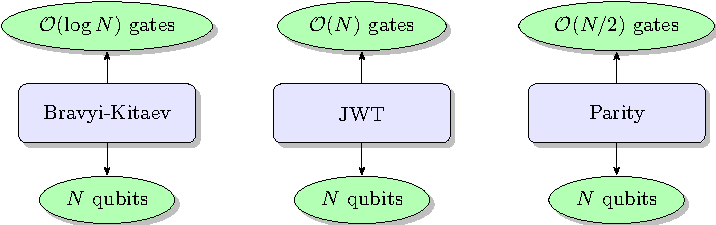
\includegraphics[width=0.7\linewidth]{Graphics/Comparaison_Mappings_Fermion-Qubit}
\caption{Comparaison des mappings fermion-qubit}
\label{fig:mappings_fermion-qubit}
\end{figure}


\subsection{Exemple : Molécule d'hydrogène}\label{sec:H2_example}

Considérons la molécure H$_2$ dans une base STO-3G. L'Hamiltonien fermionique se réduit à :
\begin{equation}
H = -1.05\ \mathbb{I} + 0.79\mathtt{Z}_0 + 0.79\mathtt{Z}_1 + 0.60\mathtt{Z}_0Z_1 + 0.20\mathtt{Y}_0\mathtt{Y}_1
\end{equation}

\begin{table}[h!]
    \centering
    \caption{Comparaison des mappings pour H$_2$ (6 qubits)}
    \begin{tabular}{lccc}
        \toprule
        \textbf{Métrique} & JWT & PT & BKT \\
        \midrule
        Nombre de termes & 14 & 11 & 9 \\
        Profondeur CNOT & 56 & 48 & 32 \\
        Fidélité & 0.992 & 0.994 & 0.997 \\
        \bottomrule
    \end{tabular}
    \label{tab:H2_comparison}
\end{table}



\section*{Exercices}

\begin{enumerate}
\item Which of the following terms is neglected in the BO approximation?
\begin{enumerate}
\item Electronic kinetic energy operator.
\item Nuclear kinetic energy operator.
\item Potential energy between the electrons and nuclei. It is the sum of all electron-nucleus Coulomb interactions.
\item Potential energy operator arising from electron-electron Coulomb repulsions.
\end{enumerate}
    
\item The Slater determinant state function is antisymmetric with respect to: 
\begin{enumerate}
\item the exchange of two electrons (permutation of two rows) 
\item with respect to the exchange of two spin orbitals (permutation of two columns)
\item both the above?
\end{enumerate}

\item Name three fermion-to-qubit transformations currently supported by Qiskit Nature.

\item Name two fermion to qubit transformations that simulate a system of electrons with the same number of qubits as electrons.

\item For which transformation does the resulting Hamiltonian commute with the number operators for spin-up and spin-down states? These operators can be utilized to taper off two qubits.
\end{enumerate}


\section*{Conclusion}

Ce chapitre a présenté les fondements théoriques et pratiques de la conversion des Hamiltoniens moléculaires en formalismes adaptés aux calculateurs quantiques. Les points clés à retenir sont :

\begin{itemize}
    \item La seconde quantification offre une représentation concise des systèmes électroniques.
    \item Les mappings fermion-qubit conservent les relations d'anticommutation.
    \item Le choix du mapping affecte directement l'efficacité du calcul quantique.
\end{itemize}

Ces concepts seront mis en pratique lors des ateliers à travers l'implémentation complète d'un algorithme VQE pour la molécule de H$_2$ sur un simulateur quantique.

\end{document}

